%%%%%%%%%%%%%%%%%%%%%%%%%%%%%%%%%%%%%%%%%%%%%%%%%%%%%%%%%%%%%%%%%%%%%%
% writeLaTeX Example: A quick guide to LaTeX
%
% Source: Dave Richeson (divisbyzero.com), Dickinson College
% 
% A one-size-fits-all LaTeX cheat sheet. Kept to two pages, so it 
% can be printed (double-sided) on one piece of paper
% 
% Feel free to distribute this example, but please keep the referral
% to divisbyzero.com
% 
%%%%%%%%%%%%%%%%%%%%%%%%%%%%%%%%%%%%%%%%%%%%%%%%%%%%%%%%%%%%%%%%%%%%%%
% How to use writeLaTeX: 
%
% You edit the source code here on the left, and the preview on the
% right shows you the result within a few seconds.
%
% Bookmark this page and share the URL with your co-authors. They can
% edit at the same time!
%
% You can upload figures, bibliographies, custom classes and
% styles using the files menu.
%
% If you're new to LaTeX, the wikibook is a great place to start:
% http://en.wikibooks.org/wiki/LaTeX
%
%%%%%%%%%%%%%%%%%%%%%%%%%%%%%%%%%%%%%%%%%%%%%%%%%%%%%%%%%%%%%%%%%%%%%%

\documentclass[letter]{article}
\usepackage{amssymb,amsmath,amsthm,amsfonts}
\usepackage{multicol,multirow}
\usepackage{calc}
\usepackage{ifthen}
\usepackage[landscape]{geometry}
\usepackage[colorlinks=true,citecolor=blue,linkcolor=blue]{hyperref}
\usepackage{graphicx}
\usepackage{float}
\usepackage{enumitem}
\usepackage{nccmath}
\usepackage[font=footnotesize]{caption}
\usepackage{pdfpages}

\ifthenelse{\lengthtest { \paperwidth = 11in}}
    { \geometry{top=.5in,left=.5in,right=.5in,bottom=.5in} }
	{\ifthenelse{ \lengthtest{ \paperwidth = 297mm}}
		{\geometry{top=1cm,left=1cm,right=1cm,bottom=1cm} }
		{\geometry{top=1cm,left=1cm,right=1cm,bottom=1cm} }
	}

\pagestyle{empty}
\makeatletter
\renewcommand{\section}{\@startsection{section}{1}{0mm}%
                                {-1ex plus -.5ex minus -.2ex}%
                                {0.5ex plus .2ex}%x
                                {\normalfont\large\bfseries}}
\renewcommand{\subsection}{\@startsection{subsection}{2}{0mm}%
                                {-1explus -.5ex minus -.2ex}%
                                {0.5ex plus .2ex}%
                                {\normalfont\normalsize\bfseries}}
\renewcommand{\subsubsection}{\@startsection{subsubsection}{3}{0mm}%
                                {-1ex plus -.5ex minus -.2ex}%
                                {1ex plus .2ex}%
                                {\normalfont\small\bfseries}}

\makeatother
\setcounter{secnumdepth}{0}
\setlength{\parindent}{0pt}
\setlength{\parskip}{0pt plus 0.5ex}
% -----------------------------------------------------------------------

\title{MEC E 331 Midterm 2 Formula Sheet}

\begin{document}
% 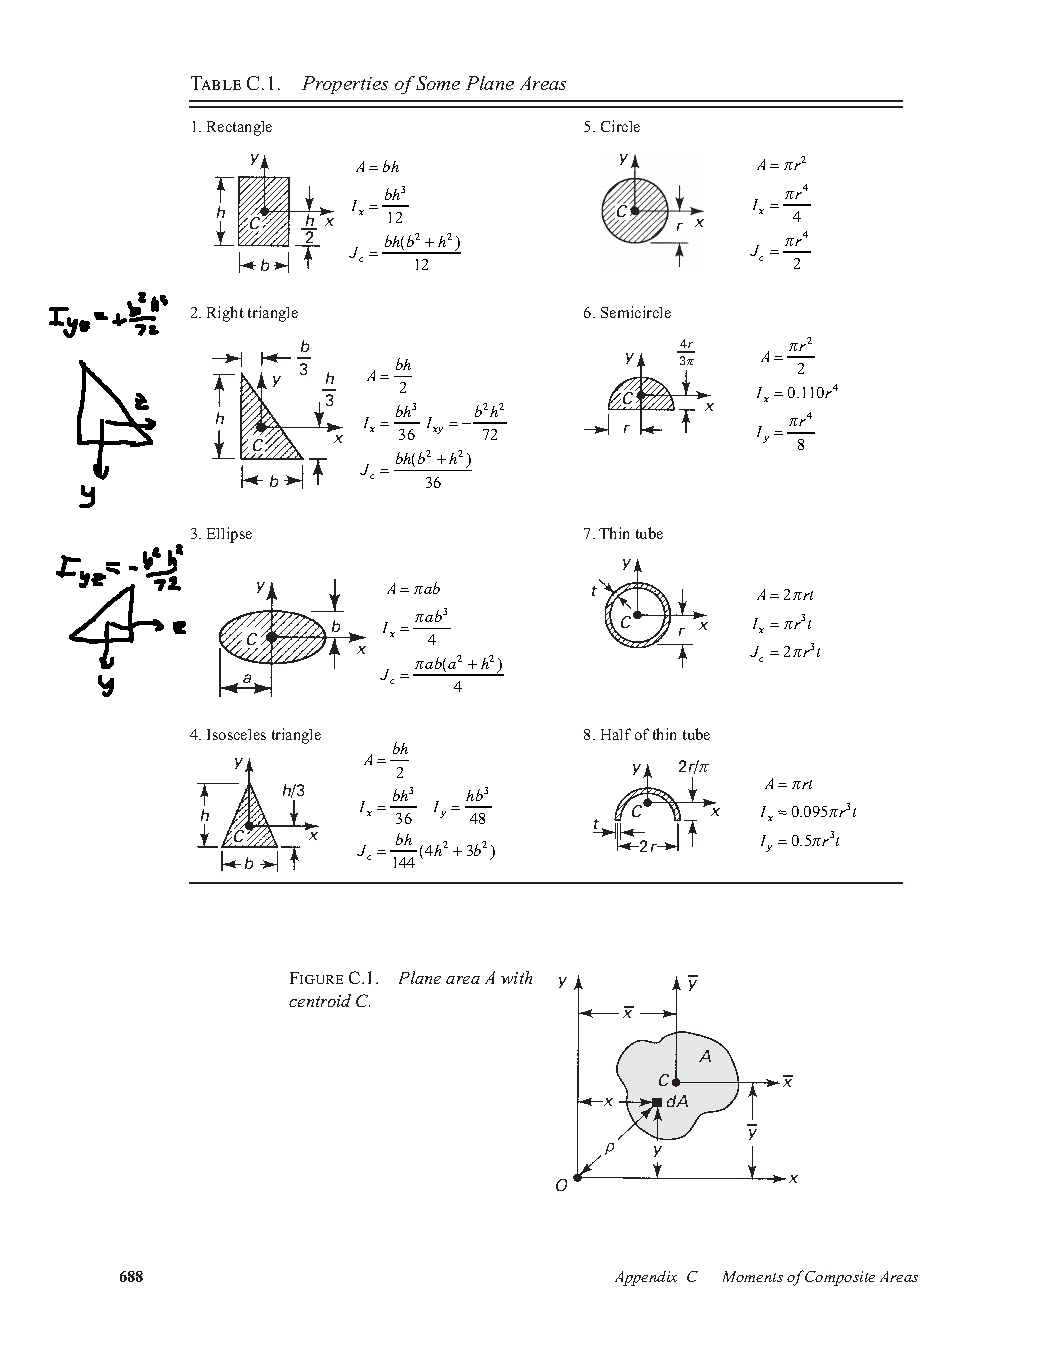
\includepdf[pages=-]{properties_of_some_plane_areas.pdf}
% 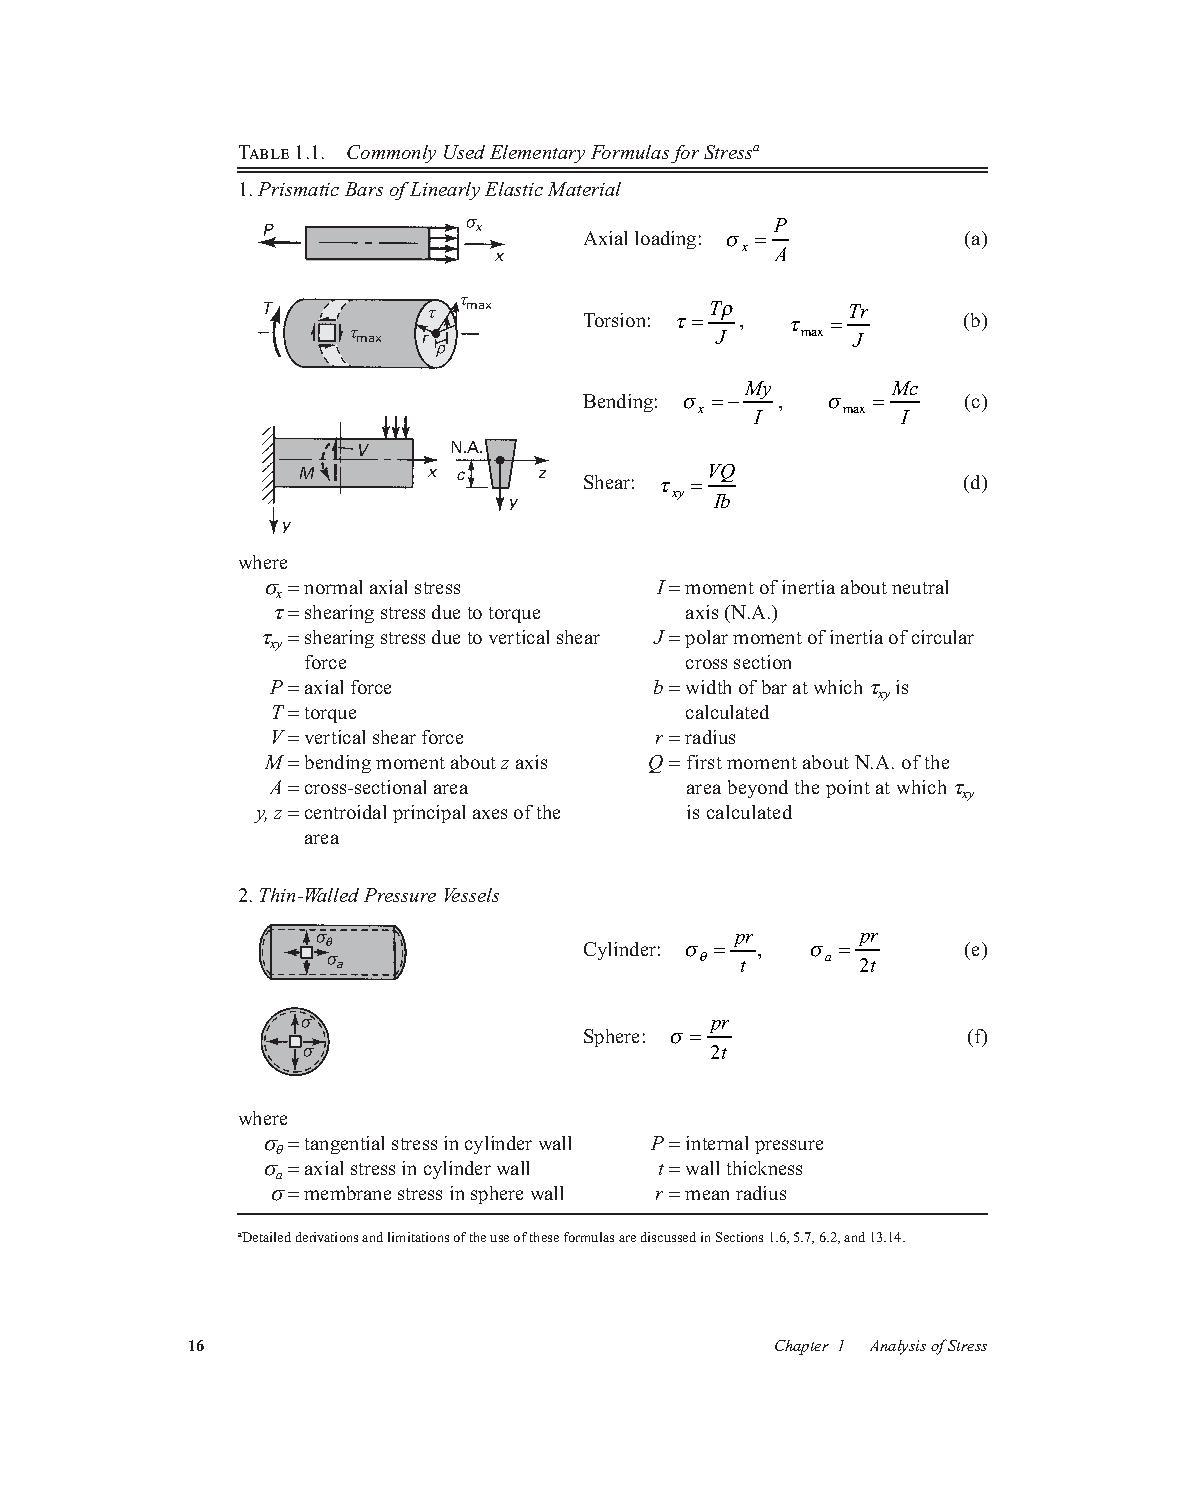
\includepdf[pages=-]{elementary_formulas.pdf}
\raggedright
\footnotesize

\begin{center}
     \Large{\textbf{MEC E 380 Quiz 4 Formula Sheet}} \\
\end{center}
\begin{multicols}{3}
\setlength{\premulticols}{1pt}
\setlength{\postmulticols}{1pt}
\setlength{\multicolsep}{1pt}
\setlength{\columnsep}{2pt}

\section*{10. Energy Methods}
Castigliano's Theorem:
Displacement
\begin{equation*}
    \delta_i = \frac{1}{EI} \int M_i \frac{\partial M_i}{\partial P_i}dx
\end{equation*}
where $P_i$ is a (dummy) concentrated load.

Angle 
\begin{equation*}
    \delta_i = \frac{1}{EI} \int M_i \frac{\partial V_i}{\partial C_i}dx
\end{equation*}
where $C_i$ is a (dummy) concentrated moment.

For polar coordinates, recall
\begin{equation*}
    \delta_i = \frac{1}{EI} \int M_i \frac{\partial M_i}{\partial P_i}rdrd\theta
\end{equation*}

\section*{3. Problems in Elasticity}
\subsection*{8.1. General Procedure}
% to do later
% \begin{enumerate}
%     \item Find fluid properties from Appendix 1 at bulk mean temperature $T_b = (T_i + T_e)/2$
%     \begin{itemize}
%         \item $\rho$, $\mu$, $k$, $c_p$, $Pr$, $\nu$
%     \end{itemize}
%     \item Determine mean velocity $V_{\text{avg}}$
%     \item Determine the type of flow (laminar or turbulent)
%     \begin{itemize}
%         \item Laminar: Re $< 2300$
%         \item Turbulent: Re $> 4000$
%     \end{itemize}
%     \item Determine the Nusselt number, Nu, using the appropriate correlation
%     \begin{itemize}
%         \item Check if $l_{h, \text{laminar}}$ and $l_{t, \text{laminar}}$ is less than $L$. If so, use Table \ref{tab:sec8_fully_developed_laminar} 
%         \item Else, use empirical correlations
%     \end{itemize}
%     \item Determine the heat transfer coefficient $h$ using $Nu$, $k$, and $A_s$
% \end{enumerate}

% % Add this to a glossary section later
% \subsection*{8.2. Variable Definitions}
% \begin{itemize}
%     \item Nu: Nusselt number
%     \item Re: Reynolds number
%     \item Pr: Prandtl number
%     \item $\mu$: Dynamic viscosity
%     \item $\nu$: Kinematic viscosity
%     \item $k$: Thermal conductivity
%     \item $h$: Convection heat transfer coefficient
%     \item $D_h$: Hydraulic diameter
%     \item $A_s$: Surface area
%     \item $A_c$: Cross-sectional area
%     \item $V_{\text{avg}}$: Average velocity
%     \item $T_b$: Bulk mean temperature
%     \item $T_i$: Inlet temperature
%     \item $T_e$: Exit temperature
%     \item $\dot{m}$: Mass flow rate
%     \item $\dot{q}$: Heat flux 
%     \item $\Delta T_{\text{lm}}$: Log mean temperature difference   
% \end{itemize}

\subsection*{8.2. Formulas}
\subsection*{Plane Strain}
On the plane $x$-$y$, the equilibrium and compatibility equations are
\begin{gather*}
    \frac{\partial \sigma_x}{\partial x} + \frac{\partial \tau_{xy}}{\partial y} = 0 \\
    \frac{\partial \sigma_y}{\partial y} + \frac{\partial \tau_{xy}}{\partial x} = 0
    \frac{\partial^2 \sigma_x}{\partial y^2} + \frac{\partial^2 \sigma_y}{\partial x^2} = \frac{\partial^2 \gamma_{xy}}{\partial x \partial y} \\
    \implies \left(\frac{\partial^2}{\partial x^2} + \frac{\partial^2}{\partial y^2}\right) (\sigma_x + \sigma_y) = 0
\end{gather*}
Strain-stress relations are
\begin{align*}
    \epsilon_x &= \frac{1}{E} \left( \sigma_x - \nu \sigma_y \right) \\
    \epsilon_y &= \frac{1}{E} \left( \sigma_y - \nu \sigma_x \right) \\
    \epsilon_z &= -\frac{\nu}{E} \left( \sigma_x + \sigma_y \right) \\
    \gamma_{xy} &= \frac{\tau_{xy}}{G} \\
    \gamma_{xz} &= \gamma_{yz} = 0 
\end{align*}
Stress-strain relations are
\begin{align*}
    \sigma_x &= \frac{E}{1-\nu^2} \left( \epsilon_x + \nu \epsilon_y \right) \\
    \sigma_y &= \frac{E}{1-\nu^2} \left( \epsilon_y + \nu \epsilon_x \right) \\
    \tau_{xy} &= G \gamma_{xy} \\
    \sigma_z &= -\frac{\nu}{1-\nu} \left( \epsilon_x + \epsilon_y \right)
\end{align*}
Airy's stress function $\Phi$ relations
\begin{gather*}
    \nabla^4 \Phi = \frac{\partial^4 \Phi}{\partial x^4} + 2 \frac{\partial^4 \Phi}{\partial x^2 \partial y^2} + \frac{\partial^4 \Phi}{\partial y^4} = 0\\
    \sigma_x = \frac{\partial^2 \Phi}{\partial y^2}, \quad \sigma_y = \frac{\partial^2 \Phi}{\partial x^2}, \quad \tau_{xy} = -\frac{\partial^2 \Phi}{\partial x \partial y}
\end{gather*}
\subsection*{Thermalelasticity}
Thermal strain, $\epsilon{t} = \alpha T$, relations by superposition,
\begin{align*}
    \epsilon_x &= \frac{1}{E} \left( \sigma_x - \nu \sigma_y \right) + \alpha T \\
    \epsilon_y &= \frac{1}{E} \left( \sigma_y - \nu \sigma_x \right) + \alpha T \\
    \epsilon_z &= -\frac{\nu}{E} \left( \sigma_x + \sigma_y \right) + \alpha T \\
    \gamma_{xy} &= \frac{\tau_{xy}}{G} \\
\end{align*}
Thermal stress relations,
\begin{align*}
    \sigma_x &= \frac{E}{1-\nu^2} \left( \epsilon_x + \nu \epsilon_y \right) - \frac{E\alpha T}{1-\nu} \\
    \sigma_y &= \frac{E}{1-\nu^2} \left( \epsilon_y + \nu \epsilon_x \right) - \frac{E\alpha T}{1-\nu} \\
    \sigma_z &= -\frac{\nu}{1-\nu} \left( \epsilon_x + \epsilon_y \right) - \frac{E\alpha T}{1-\nu} \\
    \tau_{xy} &= G \gamma_{xy} \\
\end{align*}
Stress function $\Phi$ relations,
\begin{align*}
    \left(\frac{\partial^2}{\partial x^2} + \frac{\partial^2}{\partial y^2} \right)(\sigma_x + \sigma_y + \alpha ET) &= 0 \\
    \implies \nabla^4 \Phi + \alpha E \nabla^2 T &= 0 \\
\end{align*}
\subsection*{Polar Coordinates}
Displacement-strain relations,
\begin{gather*}
    \epsilon_r = \frac{\partial u}{\partial r}, \quad \epsilon_\theta = \frac{u}{r} + \frac{1}{r} \frac{\partial v}{\partial \theta} \\
    2\epsilon_{r\theta} = \gamma_{r\theta} = \frac{\partial v}{\partial r} - \frac{v}{r} + \frac{1}{r} \frac{\partial u}{\partial \theta}
\end{gather*}
Strain-stress relations for plane stress,
\begin{gather*}
    \epsilon_r = \frac{1}{E} \left( \sigma_r - \nu \sigma_\theta \right), \quad \epsilon_\theta = \frac{1}{E} \left( \sigma_\theta - \nu \sigma_r \right)
    \epsilon_{r\theta} = \frac{1}{2G} \tau_{r\theta} \\
\end{gather*}
Airy's stress function $\Phi$ relations,
\begin{gather*}
    \sigma_r = \frac{1}{r}\frac{\partial \Phi}{\partial r} + \frac{1}{r^2} \frac{\partial^2 \Phi}{\partial \theta^2}, \quad \sigma_\theta = 
    \frac{\partial^2 \Phi}{\partial r^2} \\
    \tau_{r\theta} = \frac{1}{r^2}\frac{\partial \Phi}{\partial \theta} - \frac{1}{r}\frac{\partial^2 \Phi}{\partial r \partial \theta} = -
    \frac{\partial}{\partial r} \left( \frac{1}{r} \frac{\partial \Phi}{\partial \theta} \right)
\end{gather*}
Compatibility,
\begin{gather*}
    \nabla^2 \Phi = \frac{\partial^2 \Phi}{\partial r^2} + \frac{1}{r} \frac{\partial \Phi}{\partial r} + \frac{1}{r^2} \frac{\partial^2 \Phi}{\partial \theta^2} \\
    \nabla^4 \Phi = \left(\frac{\partial^2}{\partial r^2} + \frac{1}{r} \frac{\partial}{\partial r} + \frac{1}{r^2} \frac{\partial^2}{\partial \theta^2} \right) 
    \nabla^2 \Phi=0
\end{gather*}
Transformation equations,
\begin{align*}
    \sigma_r &= \frac{1}{2}(\sigma_x + \sigma_y) + \frac{1}{2}(\sigma_x - \sigma_y) \cos{2\theta} + \tau_{xy} \sin{2\theta} \\
    \tau_{r\theta} &= -\frac{1}{2}(\sigma_x - \sigma_y) \sin{2\theta} + \tau_{xy} \cos{2\theta} \\
    \sigma_\theta &= \frac{1}{2}(\sigma_x + \sigma_y) - \frac{1}{2}(\sigma_x - \sigma_y) \cos{2\theta} - \tau_{xy} \sin{2\theta}\\
    \sigma_x &= \frac{1}{2}(\sigma_\theta + \sigma_r) + \frac{1}{2}(\sigma_r - \sigma_\theta) \cos{2\theta} - \tau_{r\theta} \sin{2\theta} \\
    \tau_{xy} &= -\frac{1}{2}(\sigma_r - \sigma_\theta) \sin{2\theta} + \tau_{r\theta} \cos{2\theta} \\
    \sigma_y &= \frac{1}{2}(\sigma_\theta + \sigma_r) - \frac{1}{2}(\sigma_r - \sigma_\theta) \cos{2\theta} + \tau_{r\theta} \sin{2\theta}
\end{align*}
\subsection*{Concentrated Loads}
Wedge of unit thickness, under load $P$, and angle $\alpha$,
\begin{align*}
    \sigma_{r} &= - \frac{P \cos{\theta}}{r(\alpha + \frac{1}{2}\sin{2\alpha})},\quad \sigma_{\theta} = 0, \quad \tau_{r\theta} = 0\\
    \sigma_{x} &= \sigma_{r} \cos^2{\theta} = - \frac{P \cos^4{\theta}}{L(\alpha + \frac{1}{2}\sin{2\alpha})} \\
    \tau_{xy} &= \frac{P\sin\theta \cos^3\theta}L(\alpha + \frac{1}{2}\sin{2\alpha}) \\
    (\sigma_{x})_{\text{elem}} &= - \frac{P}{2L\tan{\alpha}}
\end{align*}
Note that the normal stress is maximum at $\theta = 0$ and minimum at $\theta = \alpha$. Shear stress is maximum at 
$\theta = \alpha$ if $\alpha < 30^\circ$ and at $\theta = 30^\circ$ if $\alpha \geq 30^\circ$.

\subsection*{Stress Concentrations}

For stress concentration factor $K$,
\begin{align*}
    K = \frac{\sigma_{\text{max}}}{\sigma_{\text{nom}}}
\end{align*}

\section*{5. Bending of Beams}
\subsection*{5.1. General Procedure}
General procedure of asymmetric bending problems
\begin{enumerate}
    \item Identify the location of the centroid of the cross-section, and define it as the origin of the $(y, z)$ coordinate system.
    If the centroid is unknown, set an arbitrary origin and use parallel axis theorem to find the centroid.
    \item Define the orientation of $(y, z)$ axes of the cross-section wisely so that all required moments of 
    inertia $I_y$, $I_z$, and $I_{yz}$ can be obtained (from Table) or calculated easily.
    \item Determine bending moments $M_z$ and $M_y$ at your cross-section. Use elementary beam theory to find the bending moments 
    if given a load.
    \item Use the relations to find the stress $\sigma_x$ and the neutral axis.
\end{enumerate}
\subsection*{5.2. Formulas}
Centroid equations:
\begin{align*}
    \bar{x} &= \frac{\sum \bar{x}_i A_i}{\sum A_i} 
\end{align*}
where $\bar{x}_i$ is the $x$-coordinate of the centroid of the $i$-th area, and $A_i$ is the area of the $i$-th area.

Moment equations:
\begin{gather*}
    M_y = P_z L \\
    M_z = P_y L 
\end{gather*}
where $P_z$ and $P_y$ are positive in the positive $z$ and $y$ directions, respectively.
Parallel axis theorem:
\begin{gather*}
    \bar{z} = \frac{\sum \bar{z}_i A_i}{\sum A_i} \\
    \bar{y} = \frac{\sum \bar{y}_i A_i}{\sum A_i} \\
    I_z = \sum(I_{\bar{z}, i} + A_i d_{y, i}^2) \\
    I_y = \sum(I_{\bar{y}, i} + A_i d_{z, i}^2) \\
    I_{yz} = \sum(I_{\bar{yz}, i} + A_i d_{y, i} d_{z, i}) 
\end{gather*}
where $I_{\bar{z}, i}$, $I_{\bar{y}, i}$, and $I_{\bar{yz}, i}$ are the moments of inertia about the centroidal axes, 
and $d_{y, i}$ and $d_{z, i}$ are the distances from the centroidal axes to the parallel axes. Note:
$I_{yz} = 0$ if there is symmetry about \textbf{either} the $y$ or $z$ direction.

Moment to stress:
\begin{gather*}
    \tau = \frac{VQ}{Ib} \overset{\text{rect}}{=} \frac{3V}{2A_c} \\
    \sigma_{x} = \frac{(M_y I_z + M_z I_{yz})d_{z} - (M_y I_{yz} + M_z I_y)d_{y}}{I_y I_z - I_{yz}^2} \\
    \tan{\phi} = \frac{M_y I_z + M_z I_{yz}}{M_z I_y + M_y I_{yz}} 
\end{gather*}
stress is maximum at the furthest point from the neutral axis on the cross-section. For $\sigma_x$, 
$d_y$ and $d_z$ are the signed displacements ($\pm$) from the centroid to the point of interest in the $y$ and $z$ directions.

Method of integration
\begin{align*}
    EI \frac{d^4 v}{dx^4} &= p \\
    EI \frac{d^3 v}{dx^3} &= -V \\ 
    EI \frac{d^2 v}{dx^2} &= M \\
    EI \frac{dv}{dx} &= \int M 
\end{align*}
also slope $\theta = dv/dx$ and deflection is $v$.

Singularity functions
\begin{figure}[H]
    \centering
    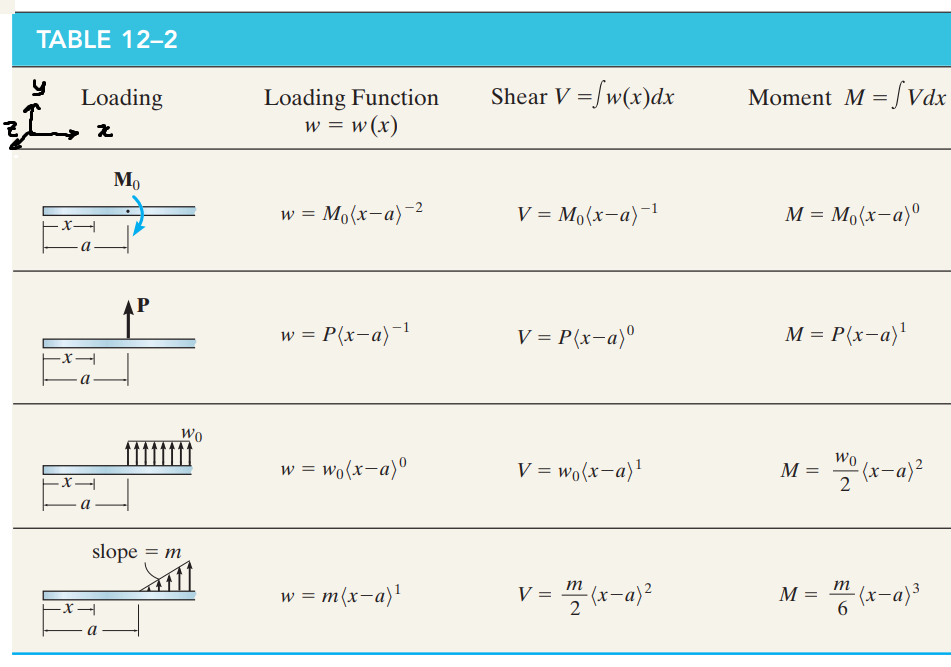
\includegraphics[width=1\linewidth]{Figures/sec5 singularity.png}
    \caption{Singularity functions}
    \label{fig:sec5 singularity functions}
\end{figure}
where 
\begin{figure}[H]
    \centering
    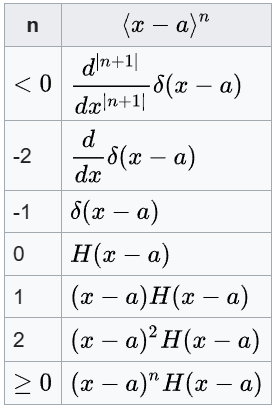
\includegraphics[width=0.5\linewidth]{Figures/sec10 singularity.png}
\end{figure}


\end{multicols}

\end{document}
